\section{Designing and Implementing Rich \Glspl{exp} with \Glspl{name}}

In this section, we describe how we design and implement \glspl{exp} for 3 languages, highlighting design inspirations and implementation details pertinent to generating helpful explanations.
In particular, we discuss techniques for natural language generation, document generation, template instantiation, and common usage mining to construct \glspl{exp} for CSS selectors, regular expressions, and \texttt{wget}.
We want to automatically create useful explanations for many different contexts without knowing those contexts ahead of time. 
Our techniques show how to automatically generate useful examples, reusing and repurposing existing documentation by reusing its codebase, and, where manual effort is needed, guide that effort to the most useful cases by extracting frequency information from the web.

\subsection{CSS}

CSS selectors appear in JavaScript, stylesheets, and even web scrapers, and despite their small size, advanced and compound CSS selectors are a frequent error for programmers working with HTML and CSS~\cite{park_towards_2013}.

\subsubsection{Explaining CSS Selectors with text}

Our method of building natural language explanations for CSS selectors involves language generation through parse tree traversal.
Our English language explanation technique starts at leaf nodes and walk up the parse treee.
First, it generates a clause at a leaf node that consists of a single noun --- the element's tag type.
At each parent, it adds a complement to the clause of an additional clause that states that the child is chosen \emph{from} the parent (Figure~\ref{alg:css_traversal}).
We map from HTML tag names to terms we expect are more understandable to those just starting with web programming --- for example, describing \texttt{a}s as `links' and \texttt{strong}s as `bolded text'. 
English language is realized using SimpleNLG\footnote{\url{https://code.google.com/p/simplenlg/}}.
Examples of text we generate to describe CSS selectors found in programming help are shown in Table~\ref{tab:css_descriptions}.

\begin{figure}
\begin{algorithmic}

\Function{visit\_node}{node}
    \If{node has id}
        clause = node.element
	\State{clause += ` with ID $node.id$'}
    \Else{}
    \State{clause = pluralize(node.element)}
    \If{node has class}
        \State{clause += ` of class $node.class$'}
    \EndIf{}
    \EndIf{}
    \If{node has child}
        \State{child = visit\_node(node.child)}
        \State{clause += child + `from' + clause}
    \EndIf{}
    \State{\Return{clause}}
\EndFunction{}

\end{algorithmic}
\caption{A recursive function for generating an explanation of a CSS selector from a tree of elements and their attributes.}
\label{alg:css_traversal}
\end{figure}

\newcolumntype{S}{>{\scriptsize\arraybackslash}m{6cm}}
\newcolumntype{T}{>{\scriptsize\arraybackslash}m{9cm}}

\begin{table*}[t]
\caption{Text Generated to Explain CSS Selectors}
\label{tab:css_descriptions}
\centering
\begin{tabular}{ST}
\toprule
\headrow{Selector} & \headrow{Realized Text} \\
\midrule
\texttt{div.video-summary-data a[href\^=/video]} & The selector `div.video-summary-data a[href\^=/video]' chooses links with URLs starting with `/video' from containers of class `video-summary-data'. \\ \midrule
\texttt{input:focus} & The selector `input:focus' chooses in-focus inputs. \\ \midrule
\texttt{p.introduction::text} & The selector `p.introduction::text' chooses text from paragraphs of class `introduction'. \\ \bottomrule
\end{tabular}
\end{table*}

\subsubsection{Generating example DOMs}

To demonstrate what CSS selectors choose, we build example HTML DOMs with elements that can be matched by that CSS selector.
We gain motivation for this \gls{exp} from the knowledge that programmers must understand the structure of the DOM before writing selectors that leverage that structure, and that this structure is most often represented through HTML\@.

Our DOM generation technique is implemented as a visitor for the parse tree our \gls{name} generates.
For each node that represent the tag of an HTML element, we use PyQuery\footnote{\url{https://pypi.python.org/pypi/pyquery}} to construct an artificial HTML element.
The visitor starts at the leaf nodes of the tree.
As it ascends, the visitor append child nodes of the parse tree as child nodes in the DOM\@.
The resulting DOM is then pretty-printed with BeautifulSoup\footnote{\url{http://www.crummy.com/software/BeautifulSoup/}}, and spaces, newlines, and carats escaped for display in the browser.

As an example, consider the \texttt{``table tr td''} selector (Figure~\ref{fig:html_table}).
The parse tree the \gls{name} produced consists of 3 nodes --- the \texttt{table} at the root, the \texttt{tr} as \texttt{table}'s only child, and \texttt{td} as the only child of \texttt{tr}.
The visitor for the CSS \gls{name} constructs an HTML node, first visiting the \texttt{td} element to generate node \texttt{<td></td>}.
It next visits the \texttt{tr} node, where it creates node \texttt{<tr></tr>} and appends the \texttt{<td></td>} element as a child.
Finally, it reaches the root node, \texttt{table}, where it constructs a \texttt{<table></table>} node and appends \texttt{<tr></tr>} as the table's child.

To convey that the leaf nodes are the elements the selector chooses (rather than all elements in the generated DOM), leaf nodes are marked with a \texttt{span} to bolden and color the element.
If an element has no tag name, we create a generic \texttt{div} to represent it.
Attributes, ids, and class names are added to the opening tag of the element.
As pseudoclasses like \texttt{checked} and \texttt{hover} are not visible from the DOM but valid components of selectors, we demonstrate their presence as comments within the element that was selected~\ref{fig:html_pseudoclass}.

Future iterations of CSS \glspl{exp} might benefit from rendering the DOMs as they would appear when viewed in a browser, particularly for inherently graphical elements like tables and form inputs.
Example DOMs that we automatically generate for real code we found in online programming help are shown in Figure~\ref{fig:selector_demonstrations}.
\if 0
\bjoern{After the submission deadline, let's revisit this technique --- I think there is a much larger design space here of showing other candidate trees that match, as well as trees that do not match. Also, we may want to indicate that selectors return collections by repeating elements --- e.g.\ td  siblings, or two different tables in the same document.}
\andrew{Roger.  Yes, I think there's a lot to do with this case of example generation.}
\fi

\begin{figure}
\centering{%
    \subfigure[\texttt{p}]{%
        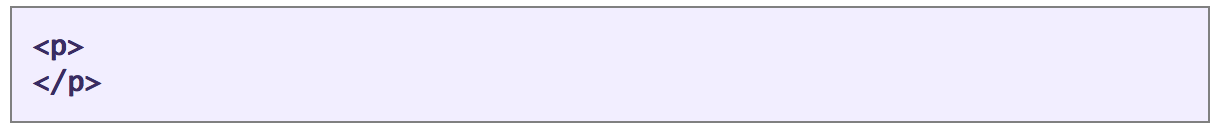
\includegraphics[width=.45\columnwidth]{figures/html_p}\label{fig:html_p}
    }
    \subfigure[\texttt{form.myform}]{%
        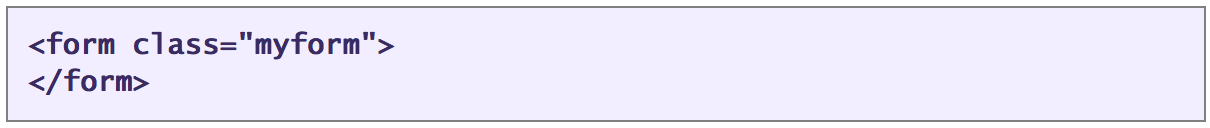
\includegraphics[width=.45\columnwidth]{figures/html_form_myform}\label{fig:html_form.myform}
    }
    \subfigure[\texttt{table tr td}]{%
        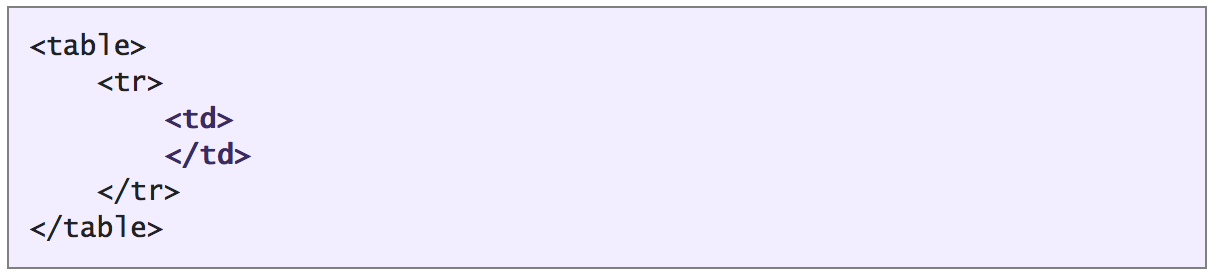
\includegraphics[width=.45\columnwidth]{figures/html_table}\label{fig:html_table}
    }
    \subfigure[\texttt{\#first:hidden}]{%
        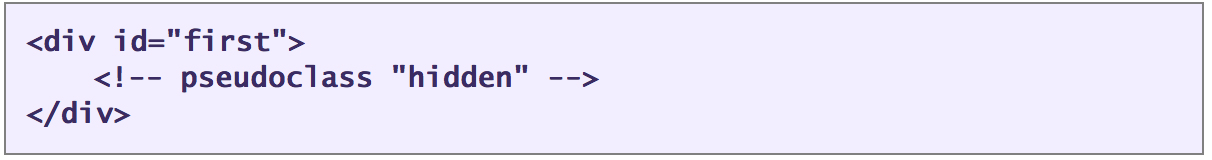
\includegraphics[width=.45\columnwidth]{figures/html_pseudoclass}\label{fig:html_pseudoclass}
    }
    \caption{Examples of HTML DOMs that can be matched by a CSS selector, automatically generated by our CSS \gls{name}.
    Note that we bolden the font of the selected node, for example in subplot~\ref{fig:html_table}, where the selected element in the \texttt{td} nested inside a \texttt{tr} in a \texttt{table}.}\label{fig:selector_demonstrations}
}
\end{figure}

\subsection{Regular Expressions}

Long regular expressions are cryptic even for expert readers to understand, leading developers to create tools to automatically generate token-by-token explanations\footnote{\url{http://rick.measham.id.au/paste/explain.pl}} and visualizations\footnote{\url{http://regexper.com/}}.
We discuss techniques for making cryptic regular expressions understandable through automatically-generated \glspl{exp} for visualizing them and generating example strings that satisfy them.

\subsubsection{Explaining Expressions through Diagrams via 3rd-Party Visualizations}

In an early prototype of a \gls{name}, we developed a regular expression \gls{name} for visualizing regular expressions, leveraging the 3rd-party regular expression visualizer called \emph{RegExper} (Figure~\ref{fig:regex_visualization}).
While the technical implementation details are trivial, we include it here as an example that a \gls{name} author can leverage demonstrations produced by his peers to create compelling \glspl{exp}.

\begin{figure}
\centering
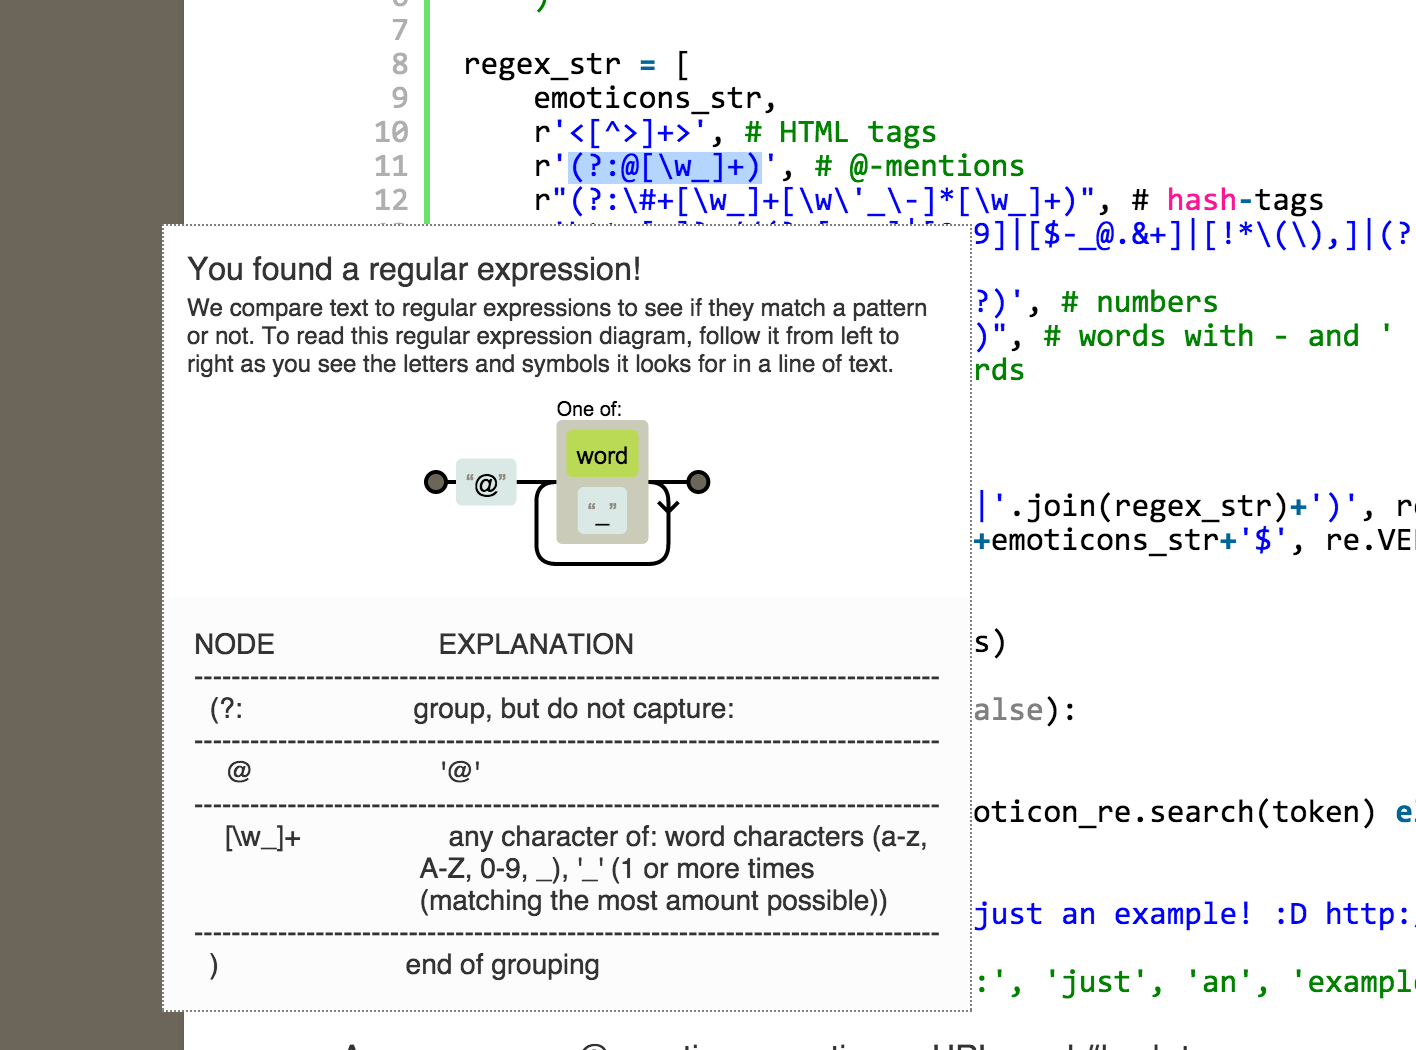
\includegraphics[width=\columnwidth]{figures/explain_on_select}
\caption{A \gls{exp} of a regular expression, adapted from the third-party tool into an in-situ tooltip \emph{RegExper}.}
\label{fig:regex_visualization}
\end{figure}

\subsubsection{Generating example expressions}

Inspired by recent work on building counterexample-guided feedback on automaton design problems~\cite{dantoni_how_2015}, we wondered, \emph{how can one generate helpful and instructive examples of what a regular expression can match?}
While we have yet to implement the detection stage of the regular expression \gls{name}, the explanation stage we have developed shares thematic ties with the CSS selector DOM generator. 
\if 0
\bjoern{Do we not have a detector because of a lack of time or because of conceptual roadblocks? Can you find all string literals in a code block, compile a regular expression for it (re.match()) and test whether that produces an error?}
\andrew{Lack of time. Sure --- I can make something that performs this.  Let me get to the preliminary study first and then move onto this.}
\fi

Like the demonstrations for CSS selectors, we choose to generate brief but demonstrative examples, assuming that strings cannot be too long, or else readers will not be able to grasp the core intent of the pattern.
Given a regular expression, we build a parse tree that consists of branches, repetitions and literals by examining output from Python's built-in regular expression compiler.
We generate each sub-pattern marked with a repetition \texttt{*} or \texttt{+} exactly once to ensure the subpattern is represented in the text without adding too much length to the string.
All literals are printed exactly as they appear in the pattern, and for simplicity, we choose the left side of each branch. 

Where we strive to make a regular expression-matching string readable is in word generation.
When we find a repetition of alphanumeric characters, we print an English dictionary word 4-6 letters in length.
If the character class contains symbols or numbers, we insert 2 random non-alphabetic characters from the class.
In this way, we insert meaningful sub-patterns based on recognizable words as the constituents from which matching strings are built.

\begin{figure}
\centering
\setlength{\fboxsep}{10pt}
\noindent\framebox[\columnwidth][c]{%
\begin{minipage}{.95\columnwidth}
\small\texttt{([0-9A-F]\{2\}[:])\{5\}([0-9A-F]\{2\})}: \\
\emph{D8:E6:0C:ED:0E:79} \\ \\
\small\texttt{\^{}(\textbackslash{}d\{3\})-(\textbackslash{}d\{3\})-(\textbackslash{}d\{4\})\$}: \\
\emph{307-039-2703}
\end{minipage}
}
\caption{Examples of strings we generate to match regular expressions.}
\label{fig:regex_strings}
\end{figure}

\subsection{wget}

The conciseness of command line options enables speedy typing, but recalling what each one does can be tricky~\cite{miller_inky_2008}.
We created a tutoron for one frequently used command line utility, the file retrieval tool \texttt{wget}, to investigate how Tutorons can explain command lines. \texttt{wget} has around 100 command line arguments, making it impractical to remember what each individual one means, particularly with its opaque short flags.
Utilities like \texttt{wget} already have comprehensive (albeit non-adaptive) documentation accessible through \texttt{man} pages and the \texttt{-h} flag from the terminal that can be used as a starting point for building in-situ documentation.
\shortchange{We focused on wget as it represents complex command lines and their problems, including argumets with meanings poorly conveyed by their symbols, and so many options to preclude recall even after extended use.}

\subsubsection{Enumerating command line options and extracting help text form source code}

We generate argument-level help for \texttt{wget} commands by extracting and modifying the short help phrases for each argument from the wget source.
Two patterns in original help messages allowed us to build more context-relevant descriptions of the arguments.
(a) Some help messages began with a noun that described what the value represented, e.g., ``location for temporary files created by the WARC writer.''
If we detected that a help phrase started with a noun using a standard typed dependency parser\footnote{\url{http://nlp.stanford.edu/software/lex-parser.shtml}}, we could add the value to the start of the statement, e.g., ``\emph{my\_dir is a} location for temporary files created by the WARC writer.''
(b) If the variable name was used in all capital letters in the help (e.g., STRING in ``insert STRING into the warcinfo record.''), we just substituted the value of the argument into the help phrase.

\subsubsection{Compound explanations of co-occurring options}

For wget, the intent of a command is often implied by a combination of options.
For examples, when \texttt{--user} and \texttt{--password} are used together, the caller is authenticating to access a restricted resource.
By using \texttt{-A}, \texttt{-r}, and \texttt{-l} together, users can recursively scrape a site for files of a certain type, to a certain depth level.

Based on a pilot effort with \texttt{wget}, we propose a way to find common use cases of commands with many options by mining programming help.
We scraped 1000 questions from StackOverflow matching the query `wget'.
From these, we extracted 510 lines of code that began with the string `wget'.
Using a custom \texttt{wget} parser from an earlier version of the \texttt{wget} \gls{name}, 346 of these lines were parsed without some lexical error.
For all lines, we then computed the co-occurrence of options, counting how often certain options were used together (Table~\ref{tab:wget_arguments}).

\begin{table}
\caption{Arguments that frequently co-occur in a sample of 500 StackOverflow posts on wget.}
\label{tab:wget_arguments}
\centering
\begin{tabular}{llc}
\toprule
\headrow{Option 1} & \headrow{Option 2} & \headrow{Count} \\
\midrule
\texttt{-r} & \texttt{-A} & 28 \\ \midrule
\texttt{--user} & \texttt{--password} & 23 \\ \midrule
\texttt{-r} & \texttt{-l} & 22 \\ \midrule
%-p & -k & 17 \\ \hline
%-r & -e & 14 \\ \hline
%-r & -P & 13 \\ \hline
%-r & -nd & 12 \\ \hline
\dots & \dots & \dots \\ \bottomrule
\end{tabular}
\end{table}

The common option combinations indeed form semantically  meaningful units. 
The combination of the \texttt{-r}, \texttt{-l<level>}, \texttt{-A<ext>}, and \texttt{-e robots=off} tags suggest that a user is about to scrape a destination URL recursively to depth level \texttt{l} for files of type \texttt{A}, without following the recommended etiquette for crawler \texttt{robots}.
In our \texttt{wget} \gls{name}, we create \emph{compound explanations}, or string templates for describing the intent of  these most-frequent groups of options, into which the values of the parameters can be substituted (Table~\ref{tab:wget_combos}).
We enforce a requirement that any one option can be described in at most one compound explanation to reduce the verbosity of text descriptions generated.
With the techniques described above, we generated explanations for \texttt{wget} command lines like those shown in Figure~\ref{fig:wget_accelerators}.

\newcolumntype{L}{>{\scriptsize\arraybackslash}m{5cm}}
\newcolumntype{C}{>{\tiny\arraybackslash}m{4cm}}
\newcolumntype{R}{>{\scriptsize\arraybackslash}m{6cm}}

\begin{table*}[t]
\caption{Templates for Describing Combinations of wget options}
\label{tab:wget_combos}
\centering
\begin{tabular}{LCR}
\toprule
\headrow{Template} & \headrow{Command} & \headrow{Realized Text} \\
\midrule
Recursively scrape web pages linked from \{url\} of type `\{accept\}', following links \{level\} times. &
\texttt{wget -l3 -A `*.jpg' \urltarget{}} & 
Recursively scrape web pages linked from http://\urltarget{} of type `*.jpg', following links 3 times. \\
\midrule
Authenticate at {url} with username `{user}' and password `{password}'. &
\texttt{wget --user andrew 
--password mypass \urltarget{}} & 
Authenticate at http://\urltarget{} with username `andrew' and password `mypass'. \\
\bottomrule
\end{tabular}
\end{table*}

\begin{figure}
\centering{%
\if 0
    \subfigure[A trivial \texttt{wget} command and an automatically-generated explanation of what it does. \bjoern{Error in figure --- commandline says ``fileurl'' but explanation says 
    ``http://fileurl'' --http isn't automatically prepended by wget. Also, you can skip the simple example if you need space.}]{%
        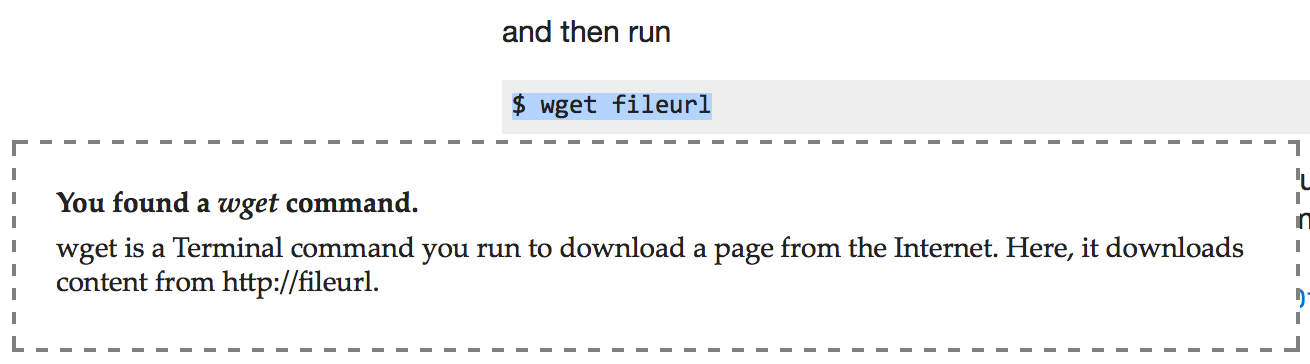
\includegraphics[width=\columnwidth]{figures/wget_trivial}\label{fig:wget_trivial}
    }
\fi
\if 0
    \subfigure[]{\label{fig:wget_complex}}
    \fi
    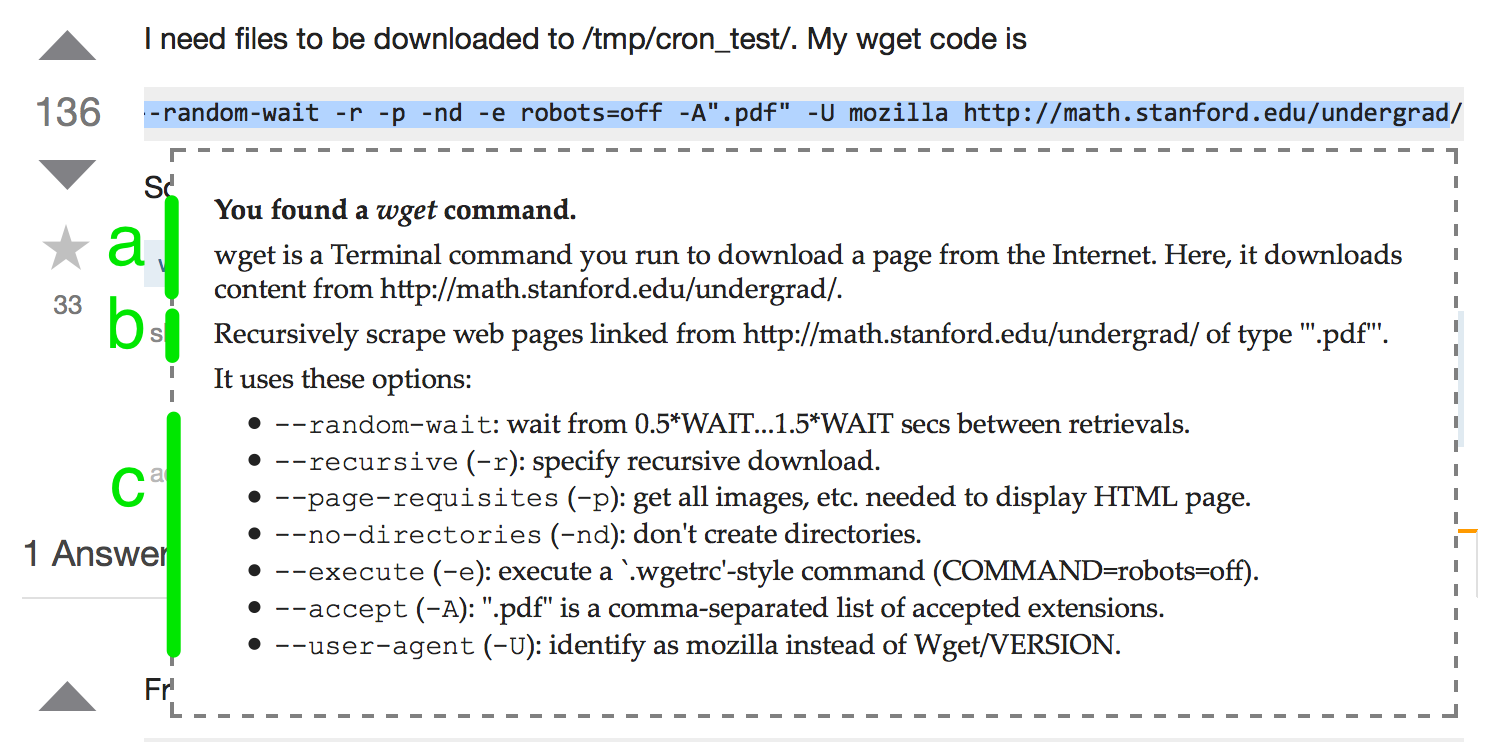
\includegraphics[width=\columnwidth]{figures/wget_complex_explained}
    \caption{%
    A multi-level explanation of \texttt{wget} comprises three parts.
        \emph{(a)} An introduction to the command.
        \emph{(b)} A meaningful description of what this combination of options does at a high level.
        \emph{(c)} A review of the meaning and values of each of the options.
    }\label{fig:wget_accelerators}
}
\end{figure}

\begin{changes}
\subsection{Design Guidelines for \Glspl{exp}}
We propose three guidelines to aid in designing \glspl{exp} for micro-languages embedded in code examples found on web pages.

First, minimize repeated text.
While our CSS natural language explanation begins with a static introduction to CSS selectors, we found that over longer usage periods, parts of the \gls{exp} that remain unchanged are likely to be ignored.
We found that 3 of the 9 participants in our usability study either commented that they were unlikely to read the introductory text as it remained unchanged, or that there was some informationt they had skimmed over that included a conceptual understanding that would have helped them.
While we have not yet concretely observed this, we suspsect that template-based explanations dependent on the arguments used are likely to be prone to similar skimming or skipping if they do not change sufficiently between very different code examples.

Second, reappropriate existing documentation.
Explanations for the wget \gls{name} were built from help strings built into the open source code for the utility.
For notoriously cryptic languages like regular expressions, many have already built visualization and explanation engines vetted by extensive community use.
The task of the \gls{name} author than becomes locating and making mashups of the parsers and explainers built by their peers to make this available to programmers in their everyday programming help searches by producing a reliable detection routine.

Third, focus on common usage.
A hand-written parser specification written in 30 lines of code successfully parsed over 99\% of CSS selectors detected in jQuery selectors, despite some simplifications of the CSS selector grammar.
Of these, 233 / 343 (67.9\%) are simple ID or class selectors.
Some features of a language are rare and therefore likely do not need to be built into first-revision parsers and explainers.
For explanations of lists of arguments, leverage usage information from the web or elsewhere, extracted with the \glspl{name} you built, to inform what greater semantic meaning can come from groups of arguments.

\end{changes}
